% Options for packages loaded elsewhere
\PassOptionsToPackage{unicode}{hyperref}
\PassOptionsToPackage{hyphens}{url}
%
\documentclass[
  ignorenonframetext,
]{beamer}
\usepackage{pgfpages}
\setbeamertemplate{caption}[numbered]
\setbeamertemplate{caption label separator}{: }
\setbeamercolor{caption name}{fg=normal text.fg}
\beamertemplatenavigationsymbolsempty
% Prevent slide breaks in the middle of a paragraph
\widowpenalties 1 10000
\raggedbottom
\setbeamertemplate{part page}{
  \centering
  \begin{beamercolorbox}[sep=16pt,center]{part title}
    \usebeamerfont{part title}\insertpart\par
  \end{beamercolorbox}
}
\setbeamertemplate{section page}{
  \centering
  \begin{beamercolorbox}[sep=12pt,center]{part title}
    \usebeamerfont{section title}\insertsection\par
  \end{beamercolorbox}
}
\setbeamertemplate{subsection page}{
  \centering
  \begin{beamercolorbox}[sep=8pt,center]{part title}
    \usebeamerfont{subsection title}\insertsubsection\par
  \end{beamercolorbox}
}
\AtBeginPart{
  \frame{\partpage}
}
\AtBeginSection{
  \ifbibliography
  \else
    \frame{\sectionpage}
  \fi
}
\AtBeginSubsection{
  \frame{\subsectionpage}
}
\usepackage{lmodern}
\usepackage{amsmath}
\usepackage{ifxetex,ifluatex}
\ifnum 0\ifxetex 1\fi\ifluatex 1\fi=0 % if pdftex
  \usepackage[T1]{fontenc}
  \usepackage[utf8]{inputenc}
  \usepackage{textcomp} % provide euro and other symbols
  \usepackage{amssymb}
\else % if luatex or xetex
  \usepackage{unicode-math}
  \defaultfontfeatures{Scale=MatchLowercase}
  \defaultfontfeatures[\rmfamily]{Ligatures=TeX,Scale=1}
\fi
% Use upquote if available, for straight quotes in verbatim environments
\IfFileExists{upquote.sty}{\usepackage{upquote}}{}
\IfFileExists{microtype.sty}{% use microtype if available
  \usepackage[]{microtype}
  \UseMicrotypeSet[protrusion]{basicmath} % disable protrusion for tt fonts
}{}
\makeatletter
\@ifundefined{KOMAClassName}{% if non-KOMA class
  \IfFileExists{parskip.sty}{%
    \usepackage{parskip}
  }{% else
    \setlength{\parindent}{0pt}
    \setlength{\parskip}{6pt plus 2pt minus 1pt}}
}{% if KOMA class
  \KOMAoptions{parskip=half}}
\makeatother
\usepackage{xcolor}
\IfFileExists{xurl.sty}{\usepackage{xurl}}{} % add URL line breaks if available
\IfFileExists{bookmark.sty}{\usepackage{bookmark}}{\usepackage{hyperref}}
\hypersetup{
  pdftitle={Charitable Giving, Tax Reform, and Political Trust},
  pdfauthor={Hiroki Kato\^{}1; Tsuyoshi Goto\^{}2; Yong-Rok Kim\^{}3},
  hidelinks,
  pdfcreator={LaTeX via pandoc}}
\urlstyle{same} % disable monospaced font for URLs
\newif\ifbibliography
\usepackage{graphicx}
\makeatletter
\def\maxwidth{\ifdim\Gin@nat@width>\linewidth\linewidth\else\Gin@nat@width\fi}
\def\maxheight{\ifdim\Gin@nat@height>\textheight\textheight\else\Gin@nat@height\fi}
\makeatother
% Scale images if necessary, so that they will not overflow the page
% margins by default, and it is still possible to overwrite the defaults
% using explicit options in \includegraphics[width, height, ...]{}
\setkeys{Gin}{width=\maxwidth,height=\maxheight,keepaspectratio}
% Set default figure placement to htbp
\makeatletter
\def\fps@figure{htbp}
\makeatother
\setlength{\emergencystretch}{3em} % prevent overfull lines
\providecommand{\tightlist}{%
  \setlength{\itemsep}{0pt}\setlength{\parskip}{0pt}}
\setcounter{secnumdepth}{-\maxdimen} % remove section numbering
\setbeamertemplate{navigation symbols}{}
\setbeamertemplate{footline}[page number]

\usepackage{bookmark}
\usepackage{booktabs}

\usepackage{xltxtra} 
\usepackage{zxjatype} 
\usepackage[ipa]{zxjafont} 
\ifluatex
  \usepackage{selnolig}  % disable illegal ligatures
\fi

\title{Charitable Giving, Tax Reform, and Political Trust}
\author{Hiroki Kato\(^1\) \and Tsuyoshi Goto\(^2\) \and Yong-Rok
Kim\(^3\)}
\date{2021/01/18}
\institute{\(^1\)Osaka University \and \(^2\)Chiba
University \and \(^3\)Kobe University}

\begin{document}
\frame{\titlepage}

\hypertarget{introduction}{%
\section{Introduction}\label{introduction}}

\begin{frame}{Background of South Korea Tax Reform}
\protect\hypertarget{background-of-south-korea-tax-reform}{}
To investigate the price effect, we use the 2014 tax reform in the South
Korea.

\begin{itemize}
\tightlist
\item
  Before 2014, tax deduction was adopted to subsidize charitable
  donation behavior.
\item
  After 2014, tax credit have been adopted.
\end{itemize}

The main difference is that tax credits reduce taxes directly, while tax
deductions indirectly lower the tax burden by decreasing the taxpayer's
marginal tax rate, which increases with gross income
\end{frame}

\hypertarget{data}{%
\section{Data}\label{data}}

\begin{frame}{National Survey of Tax and Benefit (NaSTaB)}
\protect\hypertarget{national-survey-of-tax-and-benefit-nastab}{}
\begin{itemize}
\tightlist
\item
  The Korea Institute of Taxation and Finance implements the financial
  panel survey to study the tax burden of households and the benefits
  that households receive from goverment.
\item
  The subjects of this survey are general household and household
  members living in 15 cities and provinces nationwide.
\item
  This survey is based on a face-to-face interview. If it is difficult
  for investigators to meet subjects, another family member answers on
  behalf of him.
\item
  Survey items: Annual taxable income (last year), charitable donations
  (last year), trust for politicians (5-Likert scale), and other
  covariates (age, education, gender etc.).
\item
  Survey period: 2008 \textasciitilde{} 2019

  \begin{itemize}
  \tightlist
  \item
    We use survey data after 2013 to focus on tax policy change in 2014.
  \end{itemize}
\end{itemize}
\end{frame}

\begin{frame}{Time Series of Chariable Giving}
\protect\hypertarget{time-series-of-chariable-giving}{}
\begin{figure}
\centering
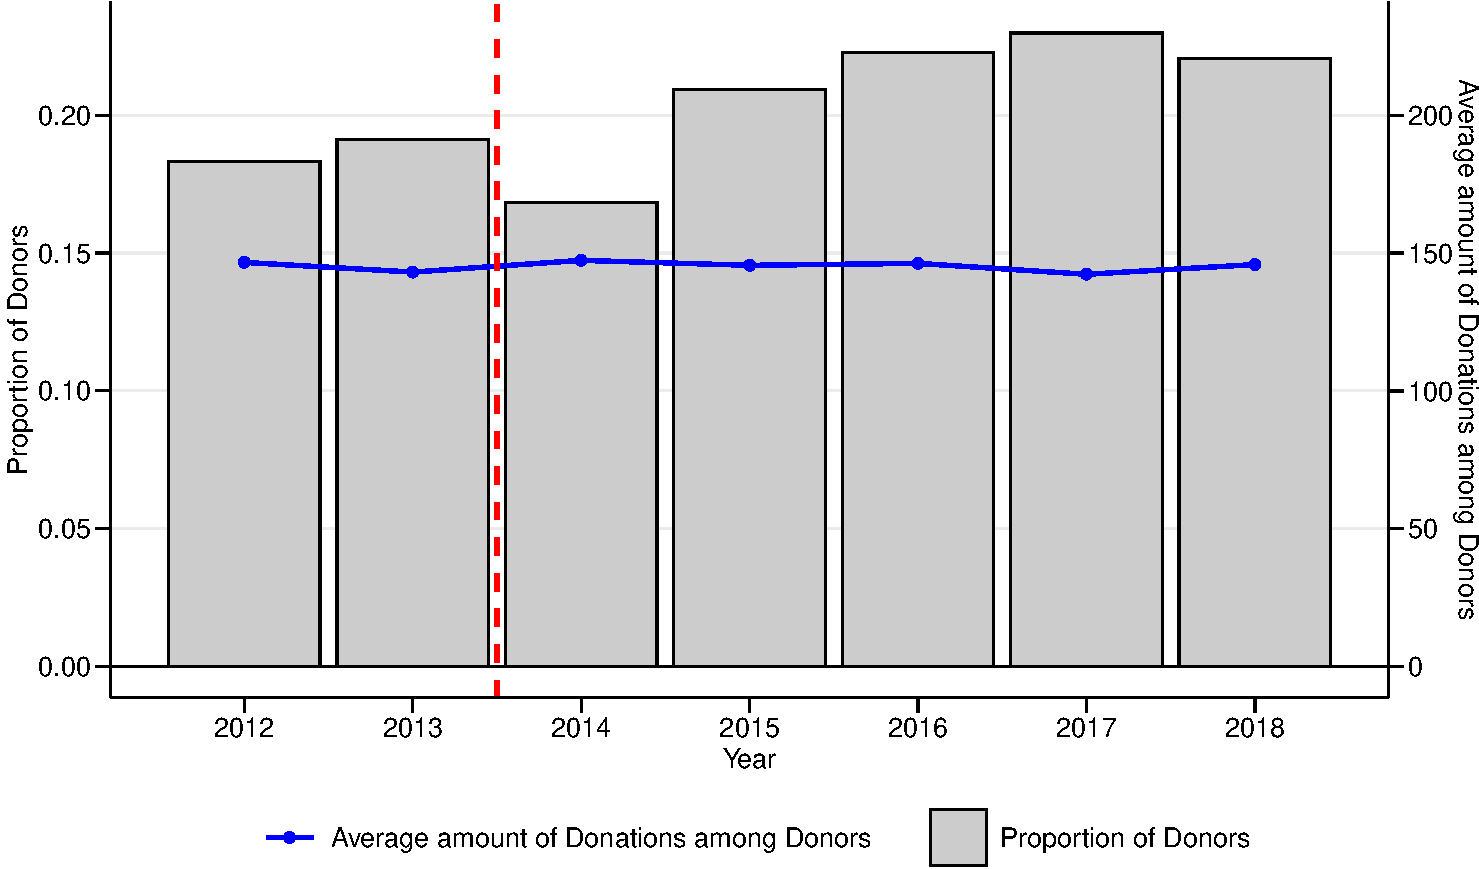
\includegraphics{C:/Users/katoo/Desktop/NASTAB/report/slides_files/figure-beamer/SummaryOutcome-1.pdf}
\caption{Proportion of Donors (bar chart) and Average Donations among
Donors (blue line)}
\end{figure}
\end{frame}

\begin{frame}{Summary Statistics of Covariates}
\protect\hypertarget{summary-statistics-of-covariates}{}
\begin{table}

\caption{\label{tab:kableSummaryCovariate}Summary Statistics of Covariates}
\centering
\fontsize{9}{11}\selectfont
\begin{tabular}[t]{lcccc}
\toprule
 & 2012 & 2013 & 2014 & 2015\\
\midrule
Female & 0.51 & 0.51 & 0.52 & 0.52\\
Age & 38.39 & 39.10 & 39.67 & 40.51\\
Annual Taxable Income & 1699.86 & 1764.04 & 1838.76 & 1872.54\\
\addlinespace[0.3em]
\multicolumn{5}{l}{\textbf{Education}}\\
\hspace{1em}Junior High School Graduate & 0.42 & 0.41 & 0.40 & 0.39\\
\hspace{1em}High School Graduate & 0.30 & 0.30 & 0.31 & 0.31\\
\hspace{1em}University Graduate & 0.28 & 0.28 & 0.29 & 0.30\\
\#.Respondents & 14138 & 13984 & 13787 & 13524\\
\#.Households & 4756 & 4807 & 4819 & 4832\\
\bottomrule
\end{tabular}
\end{table}
\end{frame}

\begin{frame}{Summary Statistics of Covariates (Cont'd)}
\protect\hypertarget{summary-statistics-of-covariates-contd}{}
\begin{table}

\caption{\label{tab:kableSummaryCovariate2}Summary Statistics of Covariates (Continued)}
\centering
\fontsize{9}{11}\selectfont
\begin{tabular}[t]{lccc}
\toprule
 & 2016 & 2017 & 2018\\
\midrule
Female & 0.52 & 0.52 & 0.52\\
Age & 41.07 & 41.89 & 42.55\\
Annual Taxable Income & 1906.91 & 1951.55 & 2039.47\\
\addlinespace[0.3em]
\multicolumn{4}{l}{\textbf{Education}}\\
\hspace{1em}Junior High School Graduate & 0.38 & 0.37 & 0.35\\
\hspace{1em}High School Graduate & 0.31 & 0.31 & 0.31\\
\hspace{1em}University Graduate & 0.31 & 0.33 & 0.34\\
\#.Respondents & 13238 & 12963 & 12795\\
\#.Households & 4790 & 4770 & 4765\\
\bottomrule
\end{tabular}
\end{table}
\end{frame}

\begin{frame}{Variable of Giving Price}
\protect\hypertarget{variable-of-giving-price}{}
In the South Korea, the tax policy about charitable giving drastically
changed in 2014. Before 2014, the \textbf{tax deduction} adpoted. After
2014, the \textbf{tax credit} adopted. Under two systems, the giving
price is

\begin{itemize}
\tightlist
\item
  tax deduction: \(\text{Price} = 1 - \tau\)
\item
  tax credit: \(\text{Price} = 1 - r\)
\end{itemize}

\(\tau\) is the marginal income tax rate calculated by annual taxable
income reported in the NaSTaB, and \(r\) is the tax credit rate
determined exogeneity. In the South Korea, \(r = 0.15\).
\end{frame}

\begin{frame}{Income Distribution and Giving Price}
\protect\hypertarget{income-distribution-and-giving-price}{}
\begin{figure}
\centering
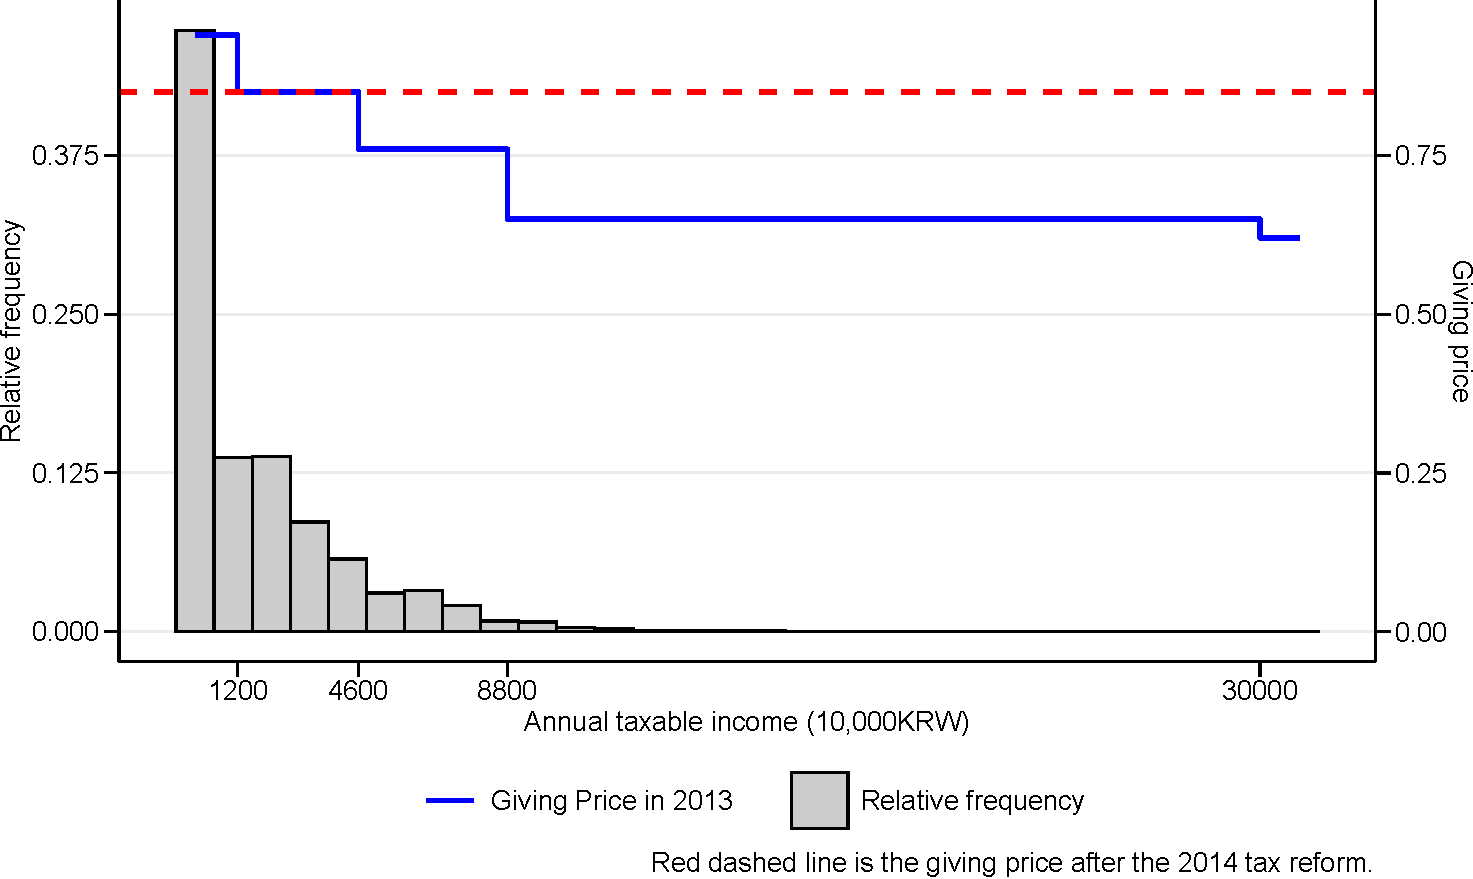
\includegraphics{C:/Users/katoo/Desktop/NASTAB/report/slides_files/figure-beamer/SummaryPriceChange-1.pdf}
\caption{Income Distribution and Giving Price}
\end{figure}
\end{frame}

\hypertarget{trust-index}{%
\section{Trust Index}\label{trust-index}}

\begin{frame}{Estimation of Trust Index}
\protect\hypertarget{estimation-of-trust-index}{}
The trust for politicans is time-varying variable because it depends on
governments' policies. We make time-invarying trust index using the
fixed effect model.

\[
    \text{Trust}_{ijt} = \text{Trustid}_{ij} + c_j \cdot \lambda_t + \lambda_t + \epsilon_{ijt}.
\]

\begin{itemize}
\tightlist
\item
  \(\text{Trust}_{ijt}\): trust for politicians (5-Likert scale)
\item
  \(\text{Trustid}_i\): individual fixed effect (\textbf{Trust index})
\item
  \(c_j \cdot \lambda_t\) captures local governments' policies effect
\item
  \(\lambda_t\) captures the central government policies effect
\end{itemize}
\end{frame}

\begin{frame}{Histrogram of Trust Index}
\protect\hypertarget{histrogram-of-trust-index}{}
\begin{figure}
\centering
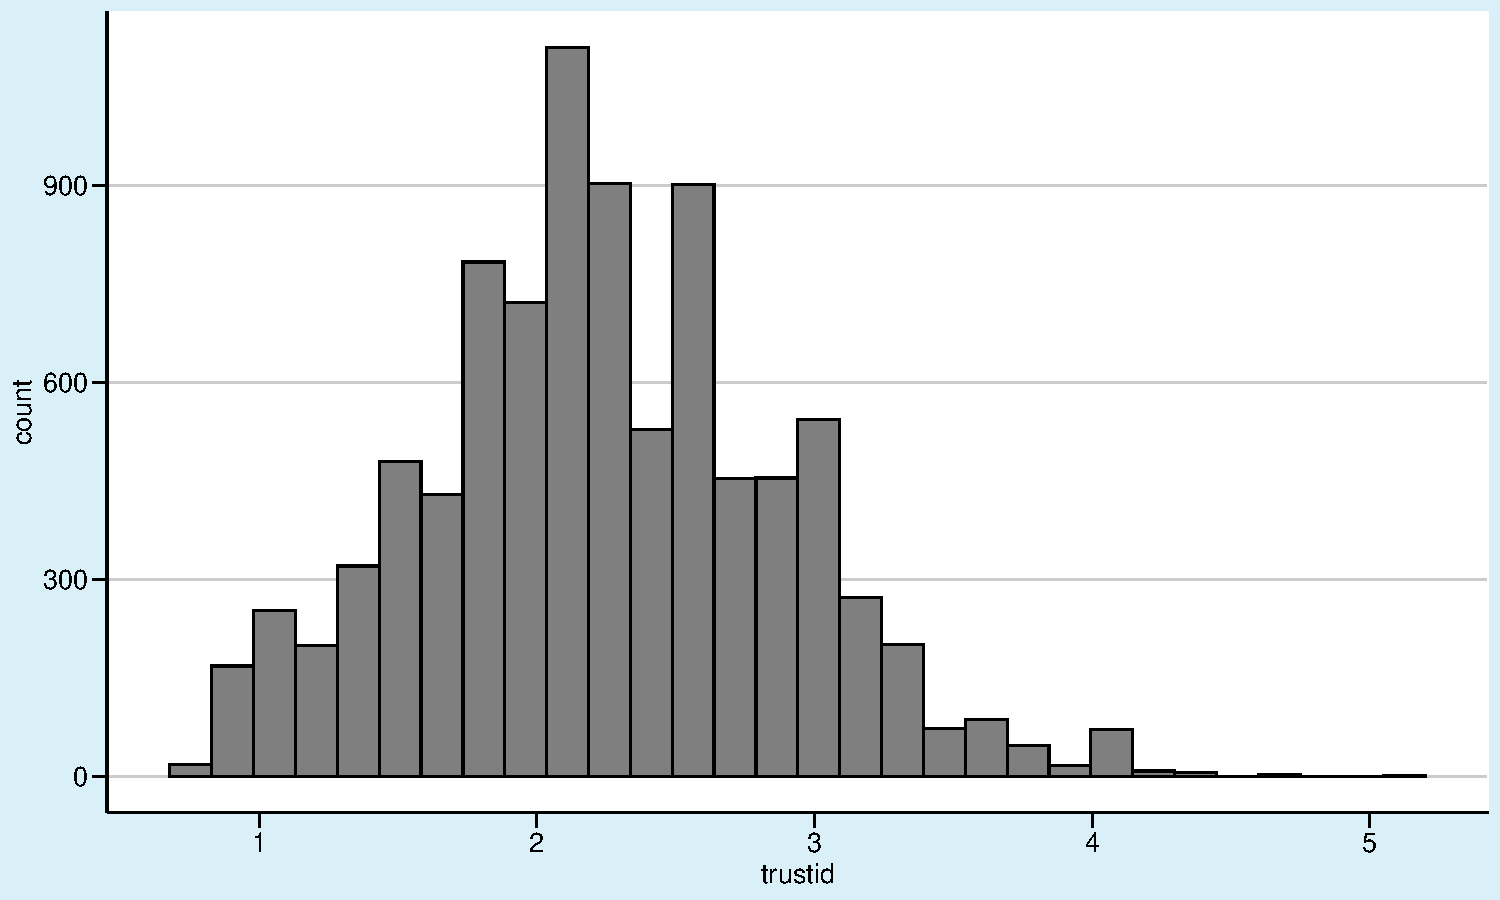
\includegraphics{C:/Users/katoo/Desktop/NASTAB/report/slides_files/figure-beamer/HistogramTrustid-1.pdf}
\caption{Histogram of Trust Index}
\end{figure}
\end{frame}

\begin{frame}{Relationship b/w Donations and Trust Index}
\protect\hypertarget{relationship-bw-donations-and-trust-index}{}
\begin{figure}
\centering
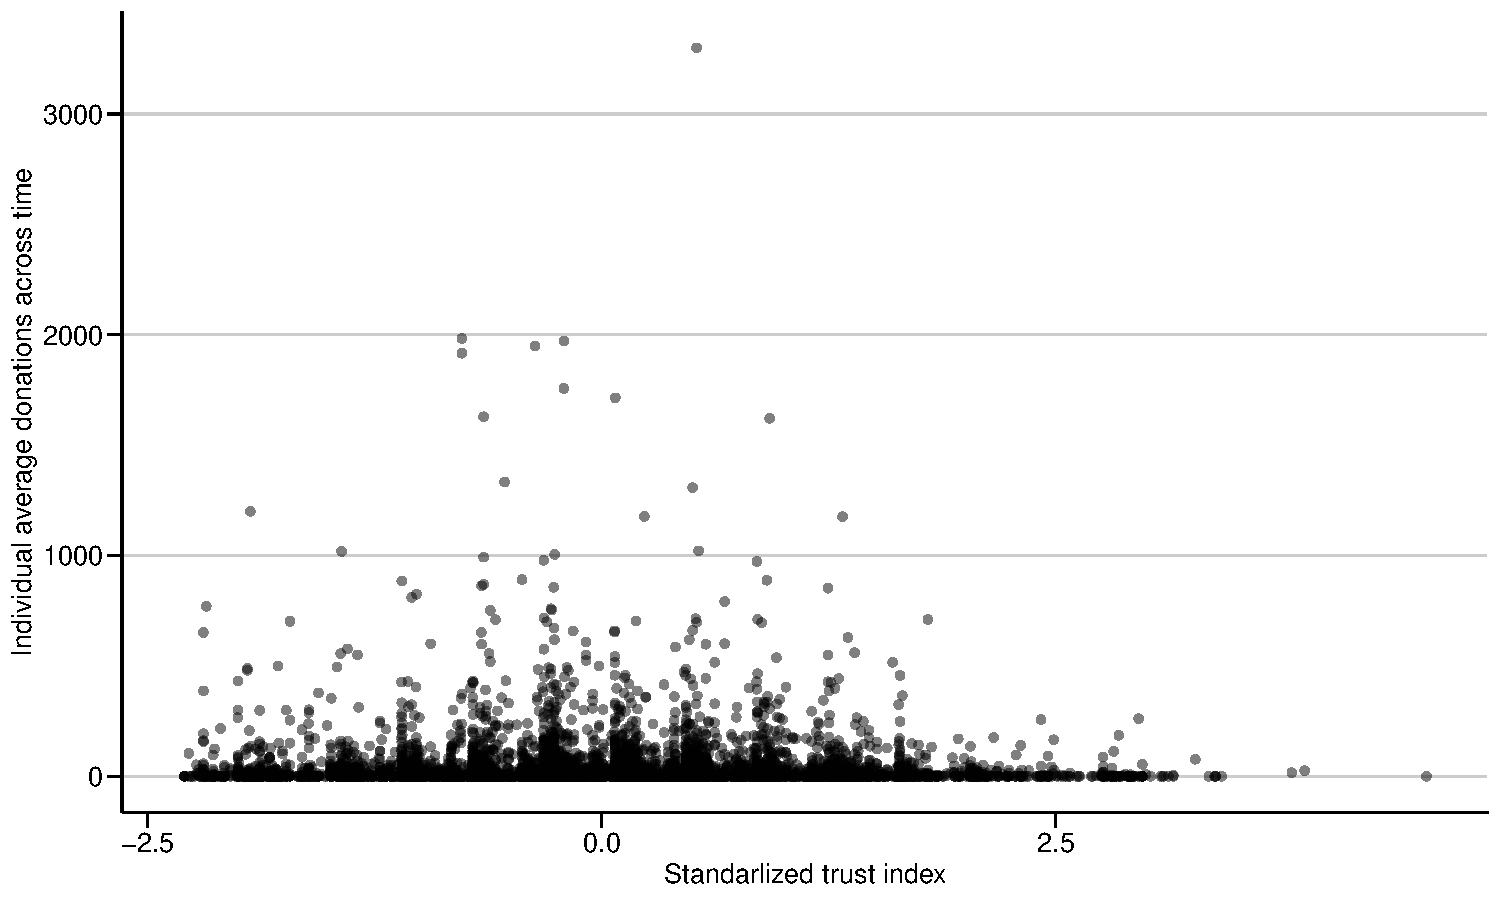
\includegraphics{C:/Users/katoo/Desktop/NASTAB/report/slides_files/figure-beamer/ScatterTrusidDonations-1.pdf}
\caption{Scatter Plot between Donations and Trust Index}
\end{figure}
\end{frame}

\begin{frame}{Relationship b/w Receving Tax Benefit and Trust Index}
\protect\hypertarget{relationship-bw-receving-tax-benefit-and-trust-index}{}
\begin{figure}
\centering
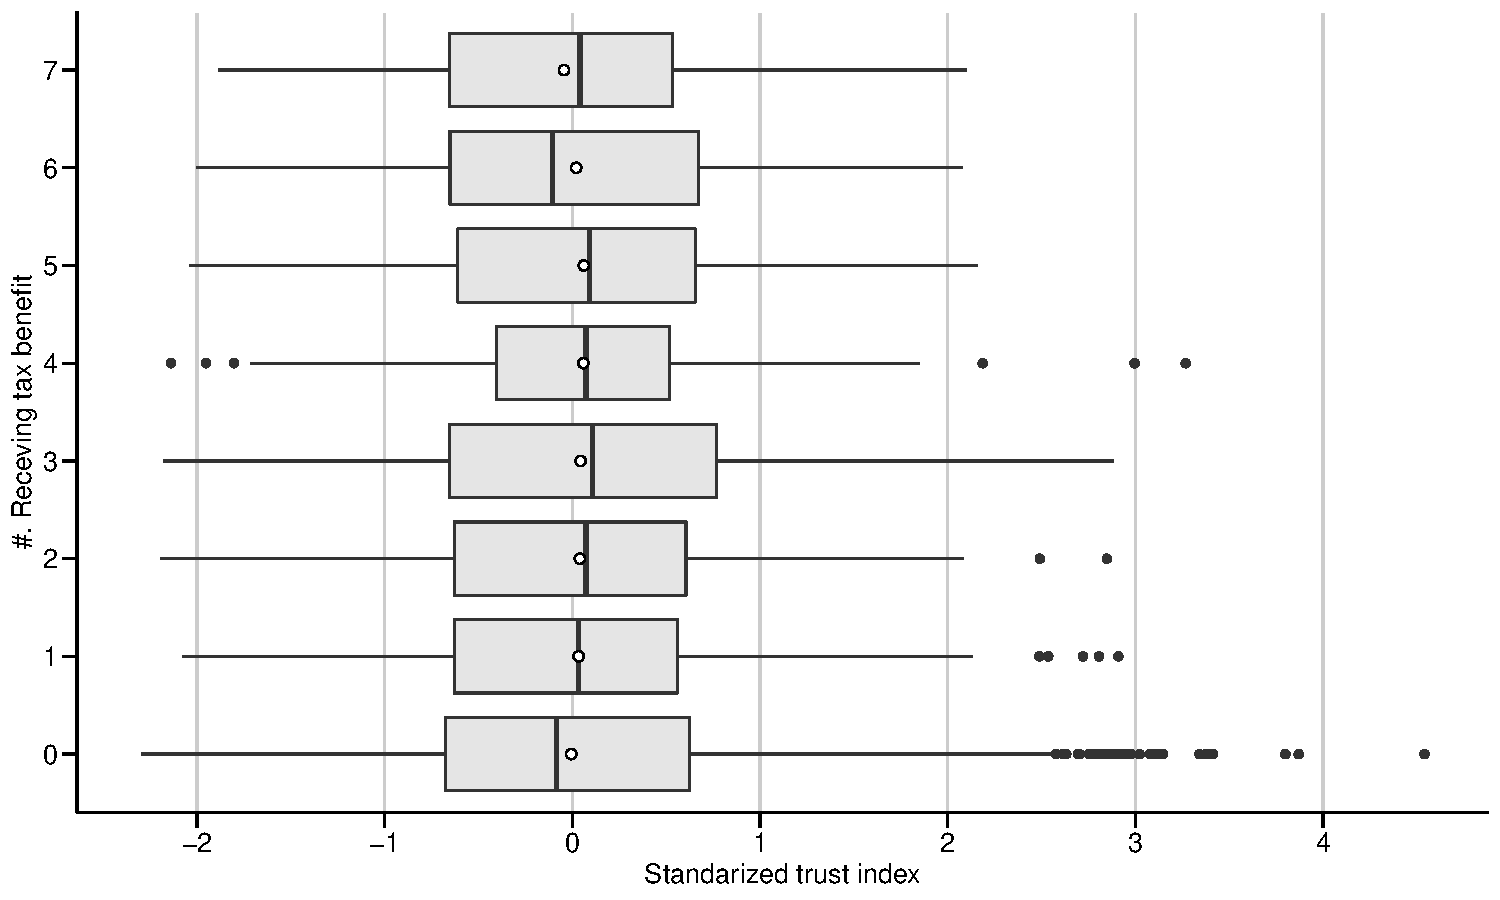
\includegraphics{C:/Users/katoo/Desktop/NASTAB/report/slides_files/figure-beamer/BoxpTrustidByBenefit-1.pdf}
\caption{Box Plot of Trust Index Grouped By Tax Benefit}
\end{figure}
\end{frame}

\begin{frame}{Regression of Trust Index on Covariates}
\protect\hypertarget{regression-of-trust-index-on-covariates}{}
\begin{table}

\caption{\label{tab:kableRegTrustidOnCovariate}Regression of Standarized Trust Index (Year = 2018)}
\centering
\begin{tabular}[t]{lcc}
\toprule
Variables & Coefficients & S.E.\\
\midrule
Female & 0.056** & (0.023)\\
Logarithm of income & 0.828* & (0.440)\\
Age & -0.022*** & (0.004)\\
squared age/100 & 0.022*** & (0.004)\\
High school graduate & 0.029 & (0.035)\\
University graduate & 0.010 & (0.038)\\
Extreme right wing & -0.224*** & (0.085)\\
Right wing & -0.036 & (0.028)\\
Left wing & -0.078*** & (0.028)\\
Extreme left wing & -0.663*** & (0.046)\\
Obs & 7697 & \\
\bottomrule
\end{tabular}
\end{table}
\end{frame}

\begin{frame}{Presidential Transition and Trust Index}
\protect\hypertarget{presidential-transition-and-trust-index}{}
In May 2017, South Korean president changed from Park Geun-hye to Moon
Jae-in. This presidential transition was due to the impeachment charge
against Park Geun-hye. People became distrustful of Park Geun-hye due to
the shinking of MV Sewol (April 2014).

Even though we control time fixed effect to estimate trust index, we are
concerned whether time fixed effect can rule out this presidential
transition effect.
\end{frame}

\begin{frame}{How to Check Presidential Transition Effect}
\protect\hypertarget{how-to-check-presidential-transition-effect}{}
To check it, we estimate trust index using both either in 2015 and 2016
(Park's Trust index) or data in 2017 and 2018 (Moon's Trust index).

Then, we carry out

\begin{enumerate}
\tightlist
\item
  t-test of difference in means between Moon's and Park's trust index
\item
  regression of the original trust index on difference in separated
  trust index
\item
  regression of the original trust index on Moon's and Park's trust
  index
\end{enumerate}
\end{frame}

\begin{frame}{Scatter Plot b/w Park's and Moon's Trust Index}
\protect\hypertarget{scatter-plot-bw-parks-and-moons-trust-index}{}
\begin{figure}
\centering
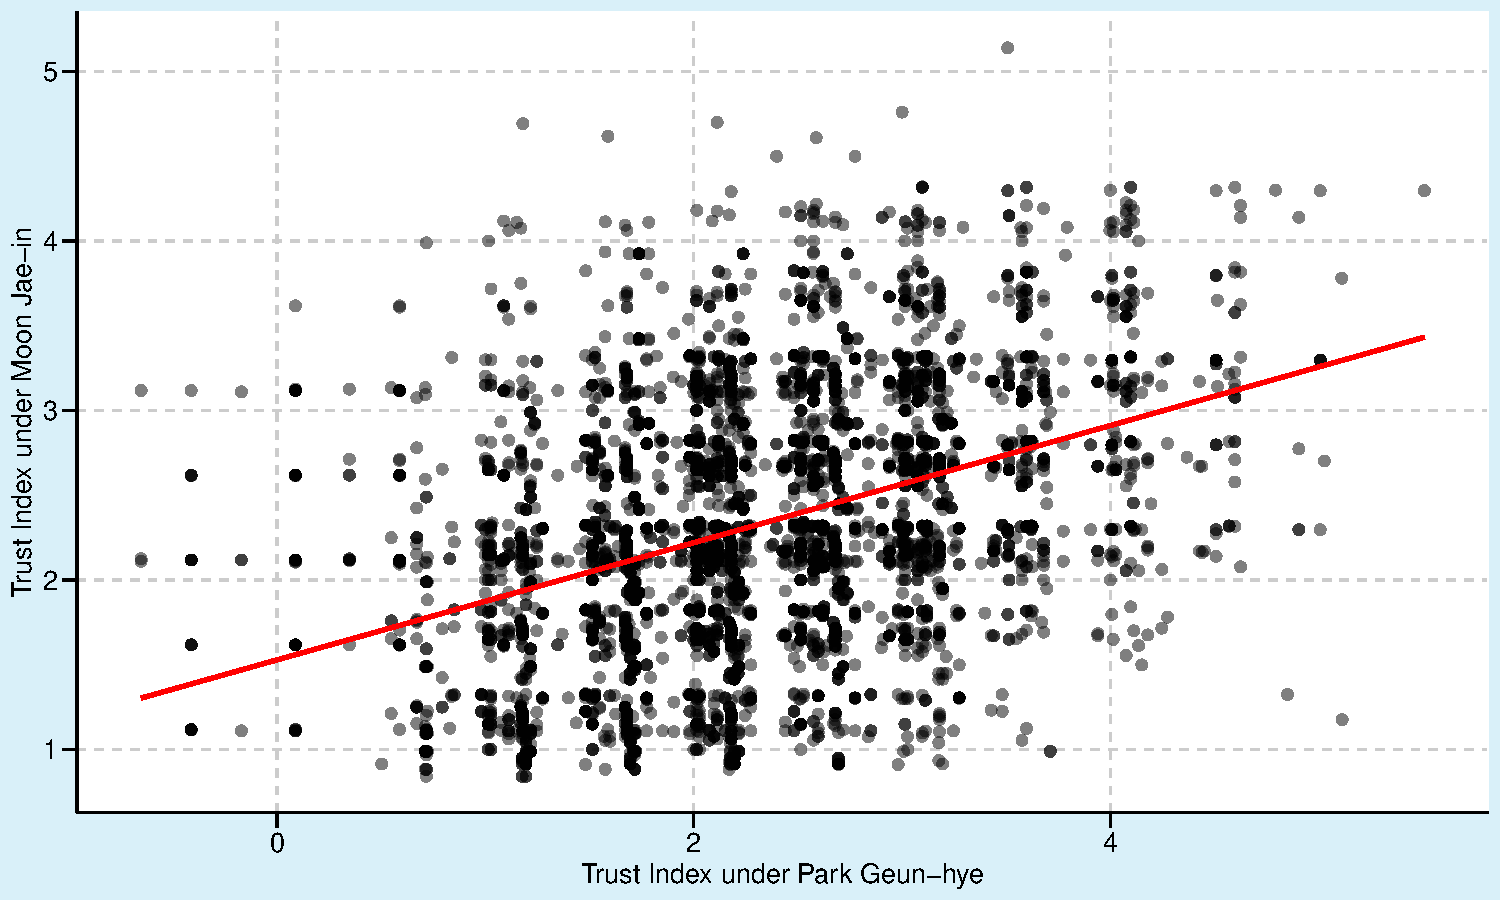
\includegraphics{C:/Users/katoo/Desktop/NASTAB/report/slides_files/figure-beamer/Scatter1Trustid-1.pdf}
\caption{Scatter Plot between Trust Index under Park Geun-hye and Moon
Jae-in}
\end{figure}
\end{frame}

\begin{frame}{Scatter Plot b/w Separated Trust Index and Original One}
\protect\hypertarget{scatter-plot-bw-separated-trust-index-and-original-one}{}
\begin{figure}
\centering
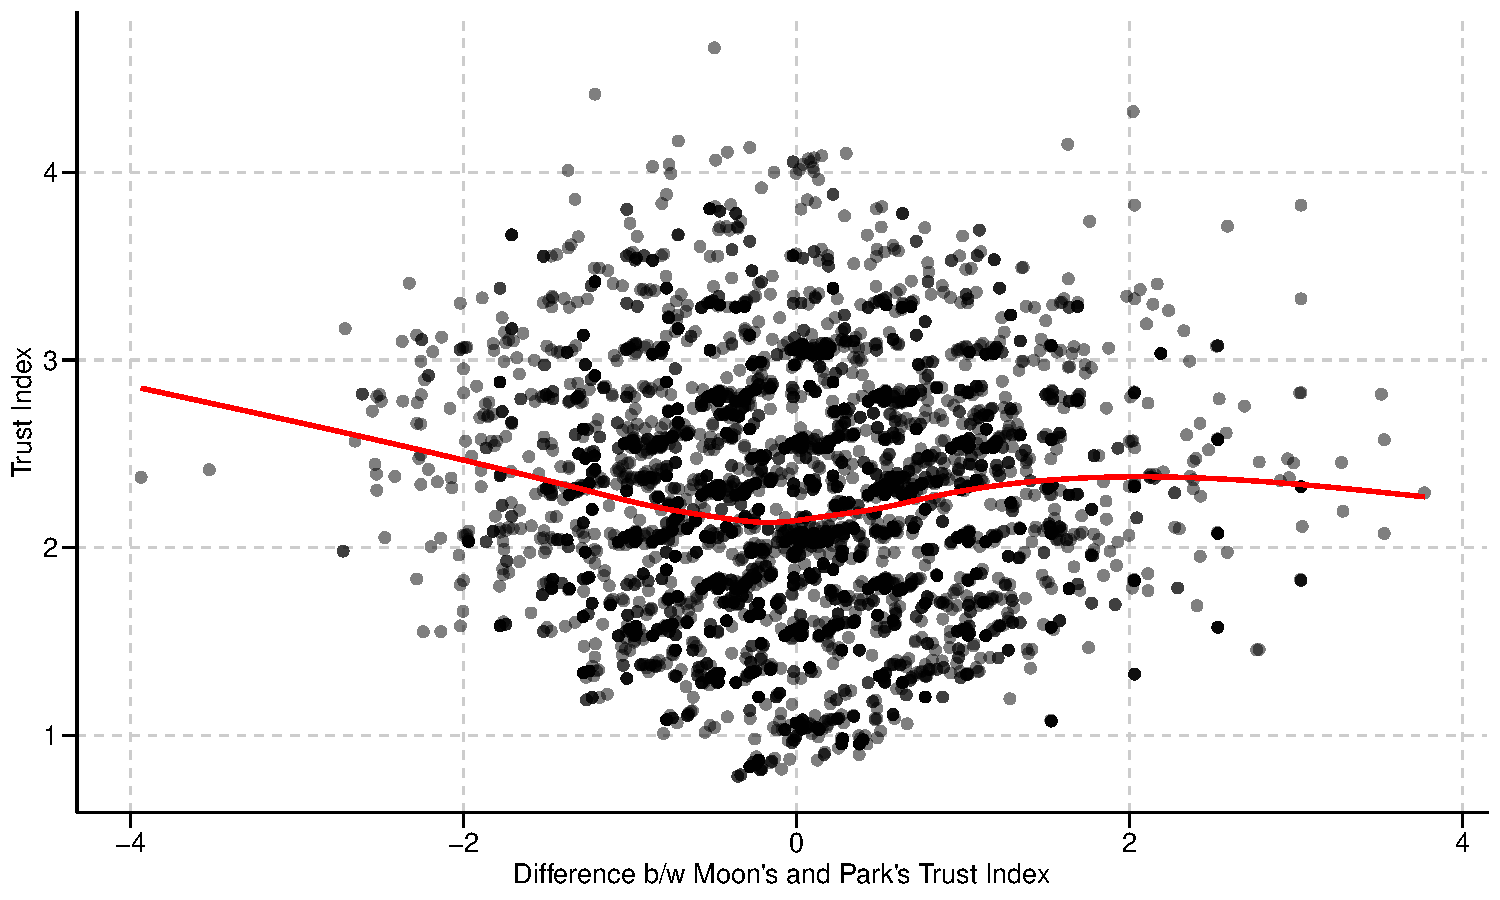
\includegraphics{C:/Users/katoo/Desktop/NASTAB/report/slides_files/figure-beamer/Scatter2Trustid-1.pdf}
\caption{Scatter Plot between Difference of Separated Trust Index and
Original One}
\end{figure}
\end{frame}

\begin{frame}{Regressions on Difference b/w President-specific Trust}
\protect\hypertarget{regressions-on-difference-bw-president-specific-trust}{}
\begin{table}

\caption{\label{tab:kableRegTrustidOnDiff2Trustid}Regressions of Trust Index on President-specific Trust Index}
\centering
\fontsize{9}{11}\selectfont
\begin{tabular}[t]{lcccc}
\toprule
 & Full & Abs < 2 & Abs < 1 & Abs < 0.5\\
\midrule
Moon's trust - Park's trust & 0.020** & 0.026*** & 0.031* & 0.035\\
 & (0.008) & (0.010) & (0.016) & (0.038)\\
Obs & 7314 & 7080 & 5666 & 3528\\
Adjusted R-sq & 0.001 & 0.001 & 0.000 & -0.000\\
\bottomrule
\end{tabular}
\end{table}
\end{frame}

\begin{frame}{Regressions on Separated Trust Index}
\protect\hypertarget{regressions-on-separated-trust-index}{}
\begin{table}

\caption{\label{tab:kableRegTrusidonSepTrustid}Regressions of Trust Index on Park's and Moon's Trust Index}
\centering
\begin{tabular}[t]{lccc}
\toprule
 & (1) & (2) & (3)\\
\midrule
Trust ID (Moon Jae-in) & 0.723*** &  & 0.574***\\
 & (0.005) &  & (0.003)\\
Trust ID (Park Geun-hye) &  & 0.521*** & 0.322***\\
 &  & (0.006) & (0.003)\\
Obs & 7314 & 7314 & 7314\\
Adjusted R-sq & 0.745 & 0.516 & 0.911\\
\bottomrule
\end{tabular}
\end{table}
\end{frame}

\hypertarget{price-elasticity}{%
\section{Price Elasticity}\label{price-elasticity}}

\begin{frame}{Baseline Regressions}
\protect\hypertarget{baseline-regressions}{}
Our baseline regression equation is

\[
    \log(\text{Giving}_{ijt}) = 
    \alpha_i + \beta_1 \log(\text{Price}_{ijt}) + \delta X_{ijt} + \lambda_t + \epsilon_{ijt}.
\]

\begin{itemize}
\tightlist
\item
  \(\log(\text{Giving}_{ijt})\) is logarithm of individual \(i\)'s
  charitable giving in year \(t\).
\item
  \(\log(\text{Price}_{ijt})\) is logarithm of individual \(i\)'s giving
  price in year \(t\).
\item
  \(\beta_1\) represents the price elasticity of giving.
\item
  \(\alpha_i\) and \(\lambda_t\) are individual and time fixed effect,
  respectively.
\end{itemize}
\end{frame}

\begin{frame}{Result of Baseline Regressions}
\protect\hypertarget{result-of-baseline-regressions}{}
We found the \textbf{price effect} of giving (1\% price increase leads
to about 1.1\% giving decrease)

\begin{table}

\caption{\label{tab:kableEstimatePElast}Baseline Regressions}
\centering
\begin{tabular}[t]{lccc}
\toprule
 & (1) & (2) & (3)\\
\midrule
ln(giving price) & -1.071*** & -1.059*** & -1.062***\\
 & (0.201) & (0.226) & (0.226)\\
Logarithm of income & Y & Y & Y\\
Age & N & Y & Y\\
Year X Educ & N & Y & Y\\
Year X Gender & N & Y & Y\\
Living Dummy & N & N & Y\\
Obs & 54213 & 54211 & 54211\\
\bottomrule
\end{tabular}
\end{table}
\end{frame}

\begin{frame}{Subgroup Regressions}
\protect\hypertarget{subgroup-regressions}{}
We estimate the baseline regression equation, using sample grouped by
the trust index.

\begin{itemize}
\tightlist
\item
  Lowest: 0 \textasciitilde{} 20\% quantile of trust index
\item
  Lower: 20 \textasciitilde{} 40\% quantile of trust index
\item
  Neutral: 40 \textasciitilde{} 60\% quantile of trust index
\item
  Higher: 60 \textasciitilde{} 80\% quantile of trust index
\item
  Highest: 80 \textasciitilde{} 100\% quantile of trust index
\end{itemize}

We include the logarithm of income, age, interactions b/w year and
education, interactions b/w year and gender, and living are dummy into
covariates.
\end{frame}

\begin{frame}{Results of Subgroup Regressions}
\protect\hypertarget{results-of-subgroup-regressions}{}
We cound \textbf{NOT} find the price effect for respondents whose trust
is very low.

\begin{table}

\caption{\label{tab:kableEstimatePElastByTrustid}Subgroup Regressions}
\centering
\fontsize{9}{11}\selectfont
\begin{tabular}[t]{lccccc}
\toprule
 & Lowest & Lower & Neutral & Higher & Highest\\
\midrule
ln(giving price) & -0.675 & -0.460 & -1.582*** & -1.284** & -1.202**\\
 & (0.556) & (0.458) & (0.481) & (0.530) & (0.503)\\
Obs & 10239 & 10358 & 10367 & 10368 & 12879\\
\bottomrule
\end{tabular}
\end{table}
\end{frame}

\begin{frame}{Heterogenity By Political Trust}
\protect\hypertarget{heterogenity-by-political-trust}{}
To capture heterogeneity precisely, we estimate the following regression
equations:

\begin{align*}
    \log(\text{Giving}_{ijt}) = 
    &\alpha_i + \beta_1 \log(\text{Price}_{ijt}) + \beta_2 \log(\text{Price}_{ijt})\cdot\text{Trustid}_{ij} \\
    &+ \delta X_{ijt} + \lambda_t + \epsilon_{ijt}.
\end{align*}

Price elasticity is obtained by
\(\beta_1 + \beta_2\cdot\text{Trust}_{ij}\).
\end{frame}

\begin{frame}{Result of Heterogeneity of Political Trust}
\protect\hypertarget{result-of-heterogeneity-of-political-trust}{}
The price elasticity is \textbf{convex} in the trust index. Those whose
trust index is low and high do not respond to the price incentive.

\begin{table}

\caption{\label{tab:kableEstimateHeteroPEstByTrusid}Heterogeneity of Political Trust}
\centering
\begin{tabular}[t]{lcc}
\toprule
 & (1) & (2)\\
\midrule
ln(giving price) & -1.108*** & -1.314***\\
 & (0.230) & (0.249)\\
\hspace{1em}X Trust index & -0.373** & -0.412**\\
 & (0.171) & (0.175)\\
\hspace{1em}X Squared trust index &  & 0.229**\\
 &  & (0.111)\\
Obs & 51306 & 51306\\
R-aq & 0.0120 & 0.0121\\
\bottomrule
\end{tabular}
\end{table}
\end{frame}

\begin{frame}{Graphical Representation of Heterogeneity Effect}
\protect\hypertarget{graphical-representation-of-heterogeneity-effect}{}
\begin{figure}
\centering
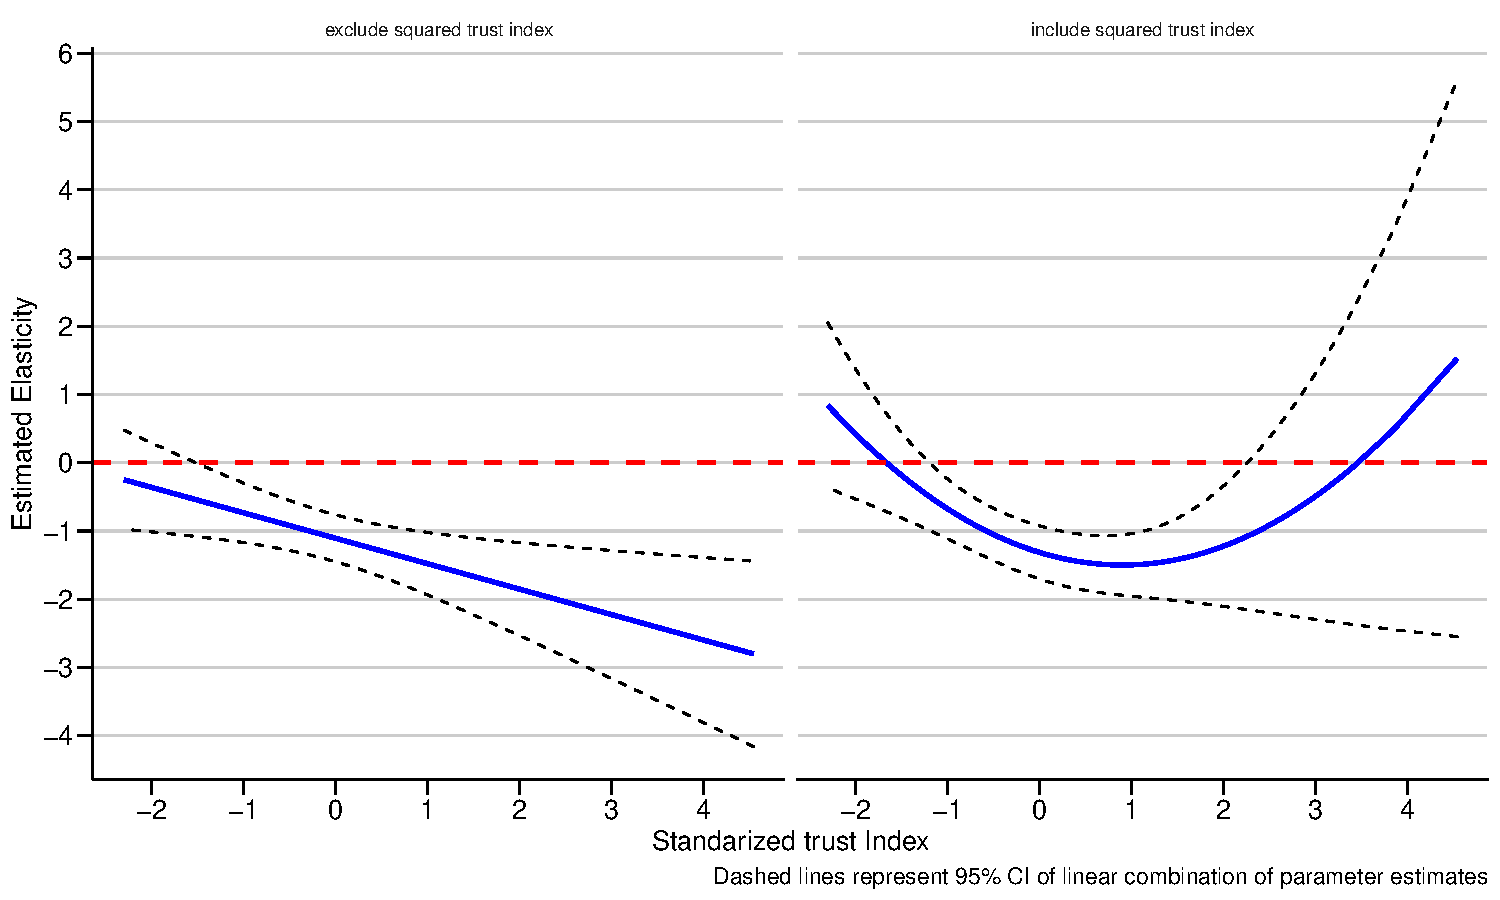
\includegraphics{C:/Users/katoo/Desktop/NASTAB/report/slides_files/figure-beamer/PlotHeteroPElast-1.pdf}
\caption{Relationship between Trust Index and Predicted Elasticity}
\end{figure}
\end{frame}

\hypertarget{conclusions}{%
\section{Conclusions}\label{conclusions}}

\begin{frame}{Conclusions}
\protect\hypertarget{conclusions-1}{}
\end{frame}

\end{document}
